\documentclass{IEEEcsmag}

\usepackage[colorlinks,urlcolor=blue,linkcolor=blue,citecolor=blue]{hyperref}
\expandafter\def\expandafter\UrlBreaks\expandafter{\UrlBreaks\do\/\do\*\do\-\do\~\do\'\do\"\do\-}
\usepackage{upmath,color}


\jvol{XX}
\jnum{XX}
\paper{8}
\jmonth{Mai}
\jname{Publication Name}
\jtitle{Publication Title}
\pubyear{2023}

\newtheorem{theorem}{Theorem}
\newtheorem{lemma}{Lemma}


\setcounter{secnumdepth}{0}

\begin{document}

\sptitle{Article Type: Description  (see Introduction for more detail)}

\title{On the maintenability of ECS and Object-Oriented programming in video games, an empirical study}

\author{ Billy Bouchard}
\affil{Polytechnique Montreal, Montreal, QC, Canada}

\markboth{THEME/FEATURE/DEPARTMENT}{THEME/FEATURE/DEPARTMENT}

\begin{abstract}\looseness-1Abstract text goes here. To find your publication's abstract\break word count limit, navigate to your magazine's homepage from\break \href{https://www.computer.org/csdl/magazines}{https://www.computer.org/csdl/magazines} and click Write for Us $>$Author Information. An abstract is a single paragraph that summarizes the significant aspects of the manuscript. Often it indicates whether the manuscript is a report of new work, a review or overview, or a combination thereof. Do not cite references in the abstract. Papers must not have been published previously and must be targeted toward the general technical reader. Papers submitted for peer review (not departments or columns) may fit into the theme of an open Call for Papers or be submitted as a ``Regular'' paper. Some Computer Society (CS) magazines provide early access to full manuscript submissions by posting a preprint of the article prior to its inclusion in an issue. Preprint articles are considered published and may be cited using their Digital Object Identifier (DOI). IEEE's Publishing Operations team will provide editorial and production services throughout the publication process.
\end{abstract}

\maketitle


\chapteri{T}he introduction should provide background information (including relevant references) and should indicate the purpose of the manuscript. Cite relevant work by others, including research outside your company or institution. Place your work in perspective by referring to other research\break papers.

% \section{LISTS}

% If you use a list, keep it short:

% \begin{itemize}
% \item[{\ieeeguilsinglright}] {\it Style for bulleted lists}---This is the style that should be used for bulleted lists.
	
% \item[{\ieeeguilsinglright}] {\it Punctuation in lists}---Each item in the list should end with a period, regardless of whether full sentences are used.

% \item[{\ieeeguilsinglright}] {\it Punctuation in lists}---Each item in the list should  end with a period.

% \end{itemize}\vspace*{3pt}


% \begin{figure*}
% \centerline{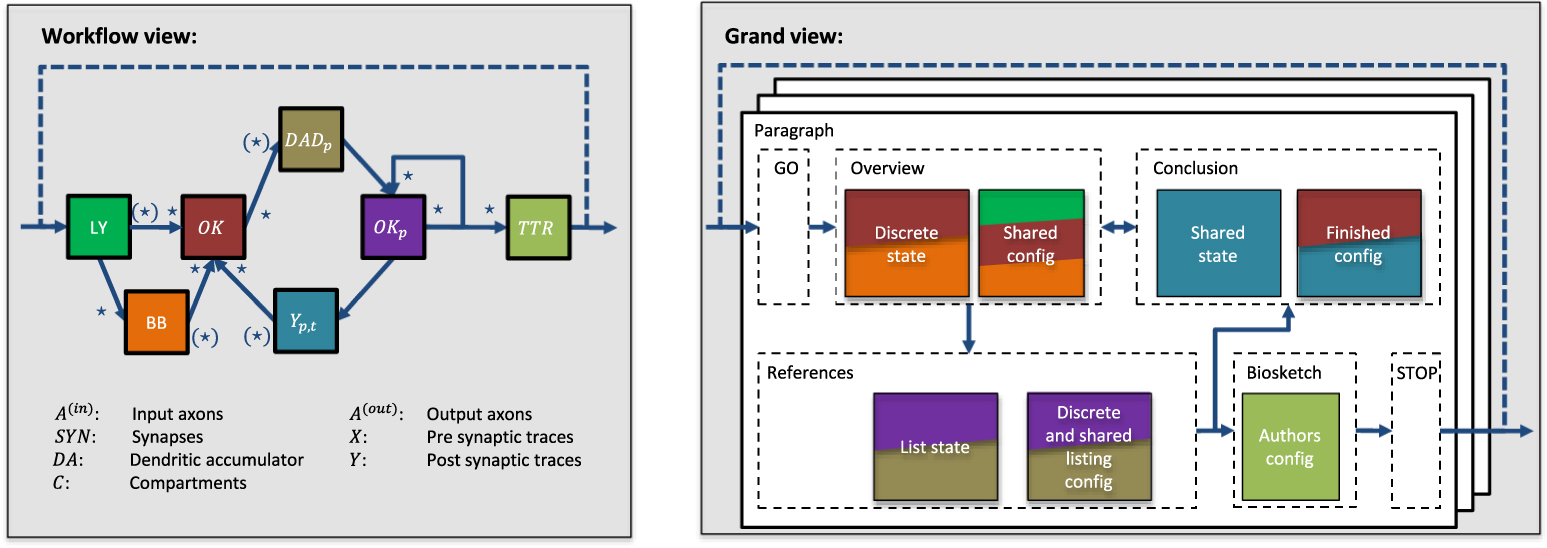
\includegraphics[width=26pc]{fig2.jpg}}
% \caption{Note that ``Figure'' is spelled out. There is a period after the figure number, followed by one space. It is good practice to briefly explain the significance of the figure in the caption. (From [``Title''],$^2$ used with permission.)}\vspace*{-5pt}
% \end{figure*}




% \section{FIGURES AND TABLES}

% \subsection{In-Text Callouts for Figures and Tables}

% Figures and tables must be cited in the running text in consecutive order. Figure callouts should be Roman, not bold or italic, like this: ``see Figure 1.'' Figure 2 shows an example of a figure spanning two columns.

% Vertical lines are optional in tables. Footnotes should be indicated by a, b, c, d, and so on, per the \emph{Chicago Manual of Style} (see Table 1). Statements that serve as captions for the entire table do not need footnote letters. 

% Authors are responsible for obtaining permission to reprint previously published figures or tables. Required permission information should be included in the figure/table caption, for instance: ``From `[Title],'$^1$ with permission,'' or ``Adapted from `[Title],'$^2$ with permission.'' \emph{Carefully} explain each figure in the text. To find your publication's figure limit, if applicable, navigate to your magazine's homepage from \href{https://www.computer.org/csdl/magazines}{www.computer.org/csdl/magazines} and click Write for Us $>$ Author Information.


\section{REFERENCE STYLE}
References must be cited in text. They appear as superscript outside the punctuation, and are listed in the References section in the order that they appear in text. Do not refer to the reference number or use ``Ref.'' or ``reference'' in text. Instead of writing ``References~3--5 show$\ldots$,'' construct the sentence independently of its reference callout; for example, ``The XYZ study shows$\ldots$.''$^{3-5}$ Please do not use automatic endnotes in Word; rather, type the reference list at the end of the paper using the ``References'' style.

Reference numbers are set flush left and form a column of their own, hanging out beyond the body of the reference. The reference numbers are on the line and end with period. In all references, the given name of the author or editor is abbreviated to the initial(s) only and precedes the last name. Include all names; use \emph{et al}. only if names are more then six. Use commas around Jr., Sr., and III in names. Abbreviate conference titles. When citing IEEE magazines or transactions, provide the issue number, page range, volume number, year, and/or month if available. When referencing a patent, provide the day and the month of issue or application. Please obtain and include relevant reference information. Do not combine references. There must be only one reference with each number. If there is a URL included with the print reference, it can be included at the end of the reference. When citing a preprint, please include the Digital Object Identifier (DOI).

Other than books, capitalize only the first word in a paper title, except for proper nouns and element symbols. For papers published in translation journals, please give the English citation first, followed by the original foreign-language citation. See the end of this document for formats and examples of common references.\vspace*{4pt}

\section{APPENDIX SECTION}

 Appendix is moved to supplementary material if it is not discussed/referenced in the main text. If it is discussed in the text, it is set as a sidebar.  


\def\refname{REFERENCES}

\begin{thebibliography}{1}

\bibitem{AA1}
G. M. Amdahl, G. A. Blaauw, and F. P. Brooks, ``Architecture of the IBM System/360,'' {\it IBM J. Res. Dev}., vol. 8, no. 2, pp. 87--101, 1964. (journal)

\bibitem{BB1}
IBM Corporation, IBM Knowledge Center - IBM Secure Service Container (Secure Service Container). [Online]. Available: {https://www.ibm.com/support/\break knowledgecenter/en/HW11R/com.ibm.hwmca.kc\_se.doc/\break introductiontotheconsole/wn2131zaci.html} (URL)

\bibitem{CC1}
J. Williams, ``Narrow-band analyzer,'' PhD dissertation, Dept.  Elect. Eng., Harvard Univ., Cambridge, MA, USA, 1993. (Thesis or dissertation)

\bibitem{DD1}
J. M. P\'erez, R. Berlanga, M. J. Aramburu, and T. B. Pedersen, ``Integrating data warehouses with web data: A survey,'' {\it IEEE Trans. Knowl. Data Eng}., early access, Dec. 21, 2007, doi:10.1109/TKDE.2007.190746. (preprint)

\bibitem{EE1}
W.-K. Chen, {\it Linear Networks and Systems}. Belmont, CA, USA: Wadsworth,  1993, pp. 123--135. (Book)

\bibitem{FF1}
S. P. Bingulac, ``On the compatibility of adaptive controllers,'' in {\it Proc. 4th Ann. Allerton Conf. Circuits Syst. Theory}, 1994,  pp. 8--16. (Conference proceedings)

\bibitem{GG1}
K. Elissa, ``An overview of decision theory,'' unpublished. (Unpublished manuscript)

\bibitem{HH1}
R. Nicole, ``The last word on decision theory,'' {\it J. Comput. Vis.}, submitted for publication. (Pending publication)

\bibitem{II1}
C. J. Smith and J. S. Smith, Rocky Mountain Research Laboratories, Boulder, CO, USA, private communication, 1992. (Private communication)
\end{thebibliography}\vspace*{-8pt}


\begin{IEEEbiography}{First A. Author}{\,}All biographies are limited to one paragraph, following the structure given here: each author's current role and institution (to match the first page of the article); three to  five current research interests; highest degree, topic, and awarding institution (do not include year); professional memberships, such as the IEEE Computer Society and any grade information; and contact information in the form of an email address.\vadjust{\vfill\pagebreak}
\end{IEEEbiography}

\begin{IEEEbiography}{Second B. Author, Jr.,}{\,} is a researcher at the  ABC Corporation, B\"oblingen, Germany.  Her current research interests include a, b, and c. Author received the Ph.D. degree  in physics from University. She is a Fellow of the IEEE Computer Society. Contact her  at sbauthor@abc.com.\vspace*{8pt}
\end{IEEEbiography}

\begin{IEEEbiography}{Third C. Author, III,} {\,} is a program officer at the  DEF Corporation, Tokyo, Japan.  His research interests include p, q, and r. Author received the Ph.D. degree  in computer vision from University. He is a member of the IEEE Computer Society. Contact him at tcauthor@def.com.
\end{IEEEbiography}

\end{document}

